\vspace{10pt}

{\centering\subsection*{贺帅:幽默的好朋友}}

\addcontentsline{toc}{subsection}{贺帅:幽默的好朋友}

\renewcommand{\leftmark}{贺帅:幽默的好朋友}

\begin{figure}[htbp]

\centering

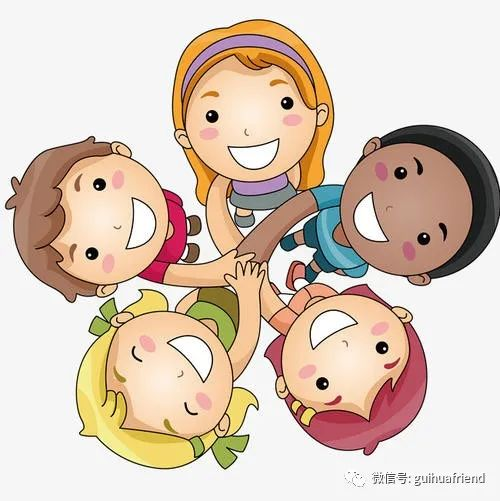
\includegraphics[width = .5\textwidth]{./ch/26.jpg}

\end{figure}





我有一个好朋友,他有一个圆圆的脑袋。一张黑黑的脸,一双水汪汪的大眼睛,最引人注目的是他的鼻子,为什么这么说呢?因为它可以控制鼻子放大再缩小。他还特别幽默。记得有一次我的好朋友在中午时给大家表演了一个节目,他自己扮成一只凶猛的狮子,又叫另一个同学扮成一只小鹿,准备好之后,节目就开始了:狮子看见肥美的小鹿,口水忍不住直流。猛的扑了过去,不仅没扑倒小鹿,自己还摔了一跤,这一家让同学们哈哈大笑。接着狮子又站了起来,用一种搞笑的声音来说:“小鹿,你逃不过我的手掌心的,我现在就要吃掉你。”说完他又扑了过去,小鹿闪开了,“哎呀”一声扑了个空。狮子觉得不能太冲动,于是他想到了一个办法,只见他偷偷混入人群中,然后趁小羊不注意,猛地扑过去,小羊就在他的面前,他也没能扑倒,并且摔了个狗啃泥,这一幕简直让我笑掉了大牙,就连伤心的同学,都被逗得破涕为笑,这一幕恰好让别的班的一个同学看到,结果好多同学都来找我说,好羡慕你们班有一个这么搞笑的同学。这就是我幽默的好朋友,我们班的开心果。你们喜欢他吗?





\vspace{10pt}



作者:五(2)班 贺帅



指导老师:周璇



投稿:2021年5月11日



发表:2021年5月12日










                



\vspace{10pt}

\hline



